\section{Лабораторная работа 6 \\
\Large Исследование напряжённо-деформированного состояния в плоской раме}

Цель работы: теоретическое и экспериментальное определение реакций опоры, перемещений и напряжений в статически неопределимой раме.

Оборудование и инструменты: специальный стенд, индикаторы перемещений часового тапа, штангенциркуль, датчик и блок измерения усилий (ИУ) цифрового типа, измеритель деформации (ИД) цифрового типа.

\subsection{Теоретические сведения}

\subsubsection{Статически неопределимая система}

\begin{figure}[!ht]
    \centering
    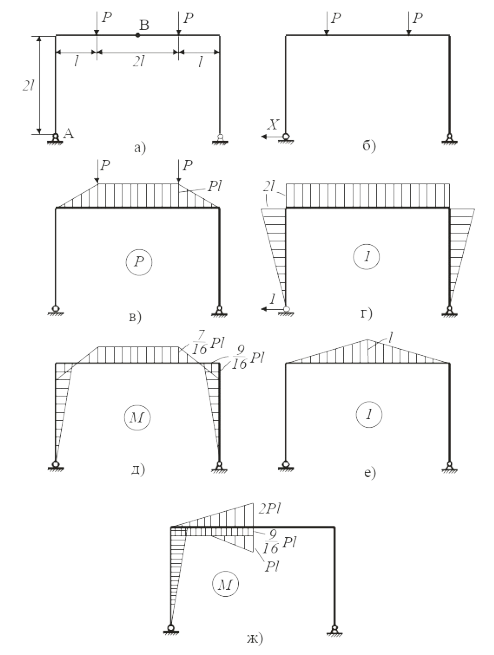
\includegraphics[width=0.8\textwidth]{static-beam}
    \caption{Раскрытие статической неопределимости плоской рамы:
        а "--- схема нагружения;
        б "--- эквивалентная схема;
        в "--- эпюра моментов от заданных сил;
        г "--- эпюра моментов от единичной силы;
        д "--- итоговая эпюра моментов;
        е "--- эпюра момента от единичной силы;
        ж "--- расчленённая эпюра моментов.
    }
    \label{fig:static-beam}
\end{figure}

Величину $X_1$ находим из канонического уравнения
\[
    \delta_{1P} + \delta_{11} X_1 = 0,
\]
которое выражает условие равенства нулю горизонтального перемещения в точке $A$.

Умножая эпюру "1" на себя, получим
\[
    \delta_{11}
    = \frac{1}{E J_X} \left(2 \cdot \frac{2 l \cdot 2 l}{2} \cdot \frac{4 l}{3} + (2 l \cdot 4 l) \cdot 2 l\right)
    = \frac{64 l^3}{3 E J_X}.
\]

Умножая эпюру "$P$" на эпюру "1", получим
\[
    \delta_{1P}
    = \frac{1}{E J_X} \left(2 \cdot \frac{P l \cdot l}{2} \cdot 2 + (P l \cdot 2 l) \cdot 2 l\right)
    = \frac{64 P l^3}{E J_X}.
\]

Находим неивестную силу и реакцию в опоре $A$:
\[
    X_1 = -\frac{9}{32} P.
\]

Изгибающий момент в сечении $B$ равен
\[
    M_B = \frac{7}{16} P l.
\]

Перемножением единичной эпюры и эпюры $M$ получим прогиб в точке $B$:
\[
    \vartheta_B
    = \frac{1}{E J_X} \cdot 2 \left(\frac{2 P \cdot 2 l}{2} \cdot \frac{2}{3} l - \frac{9}{16} P l \cdot 2 l \cdot \frac{l}{2} - \frac{P l \cdot l}{2} \cdot \frac{5}{6} l\right)
    = \frac{17}{24} \frac{P l^3}{E J_X}.
\]

Максимальные напряжения в сечении $B$ определим по формуле
\[
    \sigma_B^{\max}
    = \frac{M_B}{W_X}
    = \frac{\frac{7}{16} P l}{\frac{b h^2}{6}}
    = \frac{21 P l}{8 b h^2}.
\]

\subsubsection{Статически определимая система}

\begin{figure}[!ht]
    \centering
    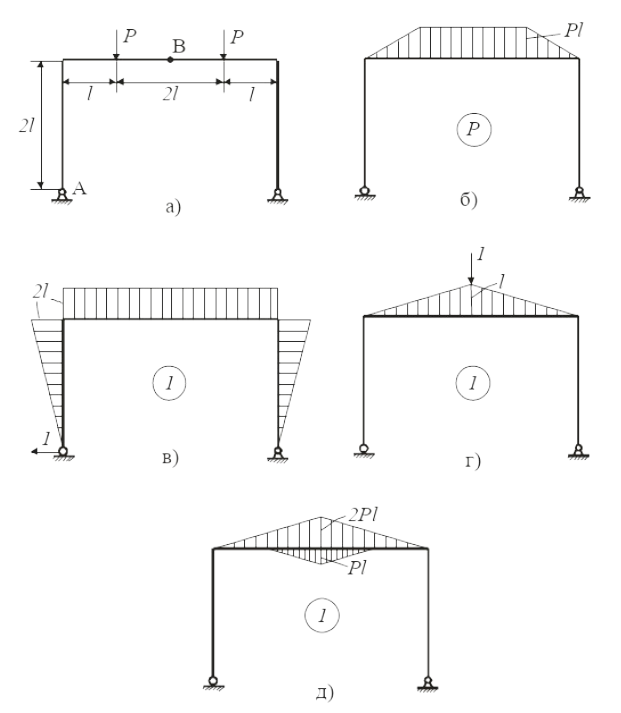
\includegraphics[width=0.7\textwidth]{static-definable-beam}
    \caption{
    }
    \label{fig:static-definable-beam}
\end{figure}

Для определения прогиба в точке $A$ удобно брать площадь эпюры $M$
\[
    \vartheta_A
    = \frac{1}{E J_X} \cdot \left(2 \cdot \frac{P l \cdot l}{2} \cdot 2 l + P l \cdot 2 l \cdot 2 l\right)
    = \frac{6 P l^3}{E J_X}.
\]

Для определения прогиба в точке $B$ эпюру $M$ удобно представить в расслоённом виде
\[
    \vartheta_B
    = \frac{1}{E J_X} \cdot 2 \cdot \left(\frac{P l \cdot l}{2} \cdot \frac{2}{3} \cdot 2 P l - \frac{P l \cdot l}{2} \cdot \frac{5}{6} l\right)
    = \frac{11}{6} \frac{P l^3}{E J_X}.
\]

Максимальные напряжения в сечении $B$ определим по формуле
\[
    \delta_B^{\max}
    = \frac{M_B}{W_X}
    = \frac{6 P l}{b h^2}.
\]

\subsection{Лабораторный стенд}

\begin{figure}[!ht]
    \centering
    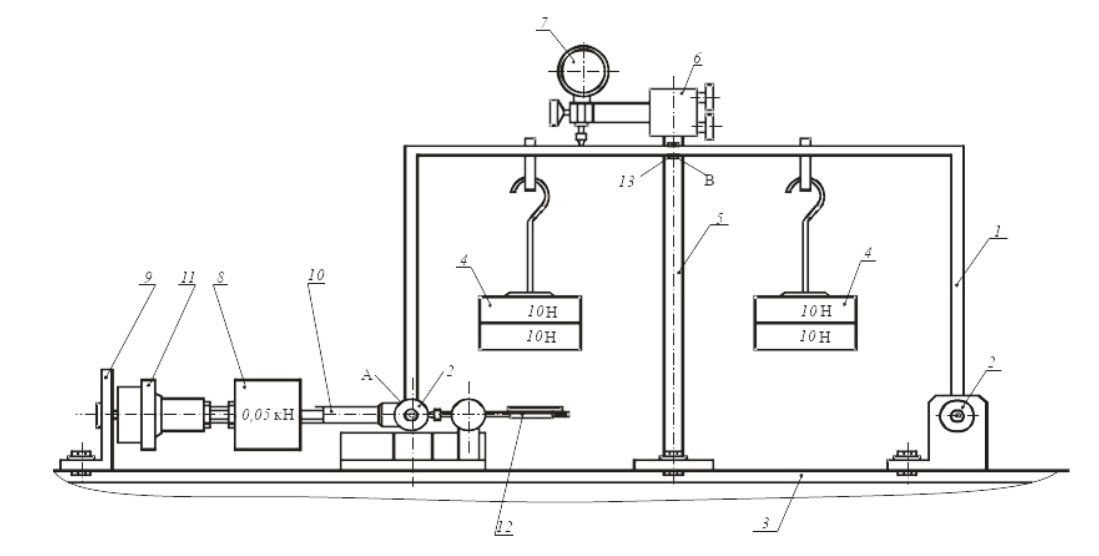
\includegraphics[width=\textwidth]{lab-bench}
    \caption{Лабораторный стенд:
        1 "--- плоская рама;
        2 "--- опорные узлы;
        3 "--- стол;
        4 "--- грузы;
        5 "--- индикаторная стойка;
        6 "--- бобышка;
        7 "---  индикатор  перемещений;
        8 "---  датчик  усилий;
        9 "---кронштейн;
        10 "--- винт датчика;
        11 "--- гайка;
        12 "--- индикатор перемещений;
        13 "--- тензодатчики.
    }
    \label{fig:lab-bench}
\end{figure}

\begin{itemize}
    \item $l = 130~мм$;
    \item $b = 30~мм$;
    \item $h = 4.5~мм$;
    \item $E = 2 \cdot 10^5~МПа$;
    \item $P = 20~Н$;
    \item $\alpha_{ед} = 10^{-6}~ед$;
    \item $\beta = 10 \cdot 10^{-2}~мм$;
\end{itemize}

\subsection{Выполнение работы}

Занесу данные в таблицу.
\begin{table}[H]
    \centering
    \caption{Напряжённо-деформированное состояние статически неопределимой рамы}
    \label{tab:static-undefinable-beam}
    \begin{tabular}{|l|c|}
        \hline
        Параметры                                                     & Результаты измерений \\ \hline
        Показание ИД верхнего тензометра в сечении $B$ при $P_0$, дел & 750                  \\ \hline
        Показание ИД нижнего тензометра в сечении $B$ при $P_0$, дел  & 620                  \\ \hline
        Показание блока ИУ в сечении $A$ при $P_0$, Н                 & 0                    \\ \hline
        Показание ИД верхнего тензометра при $P_1 = P_0 + P$, дел     & 700                  \\ \hline
        Показание ИД нижнего тензометра при $P_1 = P_0 + P$, дел      & 670                  \\ \hline
        Показание ИУ при $P_1 = P_0 + P$, Н                           & $-5.7$               \\ \hline
        Горизонтальная составляющая реакции опоры $A$, $X_1$, Н       & $-5.7$               \\ \hline
        Деформация в сечении $B$ $\epsilon_B$                         & $50 \cdot 10^{-6}$   \\ \hline
        Напряжение в сечении $B$ (погр. 12~\%) $\sigma_B$, МПа        & 10                   \\ \hline
        Показания индикатора в сечении $B$ при $P_0$, дел             & 0                    \\ \hline
        Показания индикатора в сечении $B$ при $P_1 = P_0 + P$, дел   & 68                   \\ \hline
        Прогиб в сечении $B$ $\vartheta_B$, мм                        & $0.68$               \\ \hline
    \end{tabular}
\end{table}

Имеем
\begin{align*}
    \vartheta = 0.68~мм; \\
    P = -5.62~Н; \\
    \sigma_{B \max} = 11.2~МПа; \\
    \delta = 1.4~\%.
\end{align*}

\begin{table}[H]
    \centering
    \caption{Напряжённо-деформированное состояние статически определимой рамы}
    \label{tab:static-definable-beam}
    \begin{tabular}{|l|c|}
        \hline
        Параметры                                                     & Результаты измерений  \\ \hline
        Показание ИД верхнего тензометра в сечении $B$ при $P_0$, дел & 720                   \\ \hline
        Показание ИД нижнего тензометра в сечении $B$ при $P_0$, дел  & 630                   \\ \hline
        Показание ИД верхнего тензометра при $P_1 = P_0 + P$, дел     & 605                   \\ \hline
        Показание ИД нижнего тензометра при $P_1 = P_0 + P$, дел      & 750                   \\ \hline
        Деформация в сечении $B$ $\epsilon_B$                         & $117.5 \cdot 10^{-6}$ \\ \hline
        Напряжение в сечении $B$ (погр. 12~\%) $\sigma_B$, МПа        & $23.5$                \\ \hline
        Показания индикатора в сечении $B$ при $P_0$, дел             & 0                     \\ \hline
        Показания индикатора в сечении $B$ при $P_1 = P_0 + P$, дел   & 172                   \\ \hline
        Прогиб в сечении $B$ $\vartheta_B$, мм                        & $1.72$                \\ \hline
        Показания индикатора в опоре $A$ при $P_0$, дел               & 0                     \\ \hline
        Показания индикатора в опоре $A$ при $P_1 = P_0 + P$, дел     & 567                   \\ \hline
        Прогиб опоры $B$ $\vartheta_B$, мм                            & $5.67$                \\ \hline
    \end{tabular}
\end{table}

Имеем
\begin{align*}
    \vartheta_A = \frac{6 P l^3}{E I_X} = 5.78~МПа; \\
    \vartheta_B = \frac{11 P l^3}{6 E I_X} = 1.76~МПа; \\
    \sigma_{B \max} = \frac{6 P l}{\sigma h^2} = 25.6~МПа; \\
    \delta = 8~\%.
\end{align*}

Вывод: в результате исследования НДС в плоской раме статически неопределимой системы нашёл напряжение и прогиб в точке $B$ и реактивную силу в точке $A$, после чего определил погрешность.
В статически определимой раме нашёл перемещение опоры $A$ и прогиб и напряжение в точке $B$.
Причинами погрешности являются трение в опорах, погрешность тензодатчиков, погрешность ИД.
